We evaluated our technique in phases. First, we generated data that
validates the correctness of the model, then we evaluated a small portion of
the dataset, and finally evaluated on the full dataset.

\subsection{Generated Data}
The core algorithm relies on finding a $P$ and $Q$ matrix that relate users and
businesses to latent factors (the columns of $P$ and $Q$).  Figuring out
specifically how a user $u$ feels about a business $b$ is just a matter of
taking the dot product of $P_u$ and $Q_b$.  Therefore, we started evaluation by
randomly generating a $P_{0}$ and $Q_{0}$ matrix, and then creating the rating table
by multiplying the matrices. Running our algorithm on this data yielded similar
$P$ and $Q$ matrices, which indicated that the algorithm was doing
what we expected it to do as a sanity check.

\subsection{Yelp Data}
In order to show just how effective
our model is, we needed to evaluate on the actual businesses data from Yelp. We
started evaluation by taking dense chunks of data from the Yelp set. Thus, we'd
only have a couple hundred ratings.
This step was critical to expose inefficiencies in our calculations. Indeed,
once we started doing this, we immediately realized the need to switch the core of our code
from Python to a C++ module.

To evaluate our algorithm on a dataset, we used 5-fold cross-validation. To do
this we placed each rating into a random fold, giving us 5 folds of
approximately the same size. Then we pick a fold to call the infold, and call
all of the data not in that fold the outfold. To measure how well our algorithm
worked, we generated a $P$ and $Q$ on all of the ratings in the outfold. We
calculated distance by generating a predicted rating for each item in the
infold, taking the distance and squaring it. We then average the distance squared for
every rating in the infold and call this the Residual Sum of Squares (RSS). We
present our data as a Root Mean Squared Error (RMSE) to give an idea of the actual
average distance between predicted ratings and actual ratings.

For training, we removed California's businesses ratings from the Yelp data
set. This meant removing roughly \numBusCA businesses from \numBusTotal total
businesses and \numRatingCA from \numRatingTotal ratings.
The red line in Figure~\ref{fig:nocal} shows a plot of RMSE vs. K for all data excluding
California's. For the evaluation step, we ran our algorithm on ratings for
California businesses only. The red line in Figure~\ref{fig:cal} shows a plot of RMSE vs. K for
ratings only on California businesses. No parameters were changed between the
training and evaluation run. The graphs show that the K-values have roughly the
same effect on RMSE in both cases. Thus, a K-value that gives a good RMSE value
in the data excluding California gives a good RMSE value in the data for
California. This result indicates that our model works well on
data which we did not train or tune with. This also indicates that it might be
possible to make assumptions about the number of factors people use when
deciding what businesses they like. Because of this, we can
pick a K that gives good results across most realistic datasets.

\begin{figure}[ht!]
	\centering
	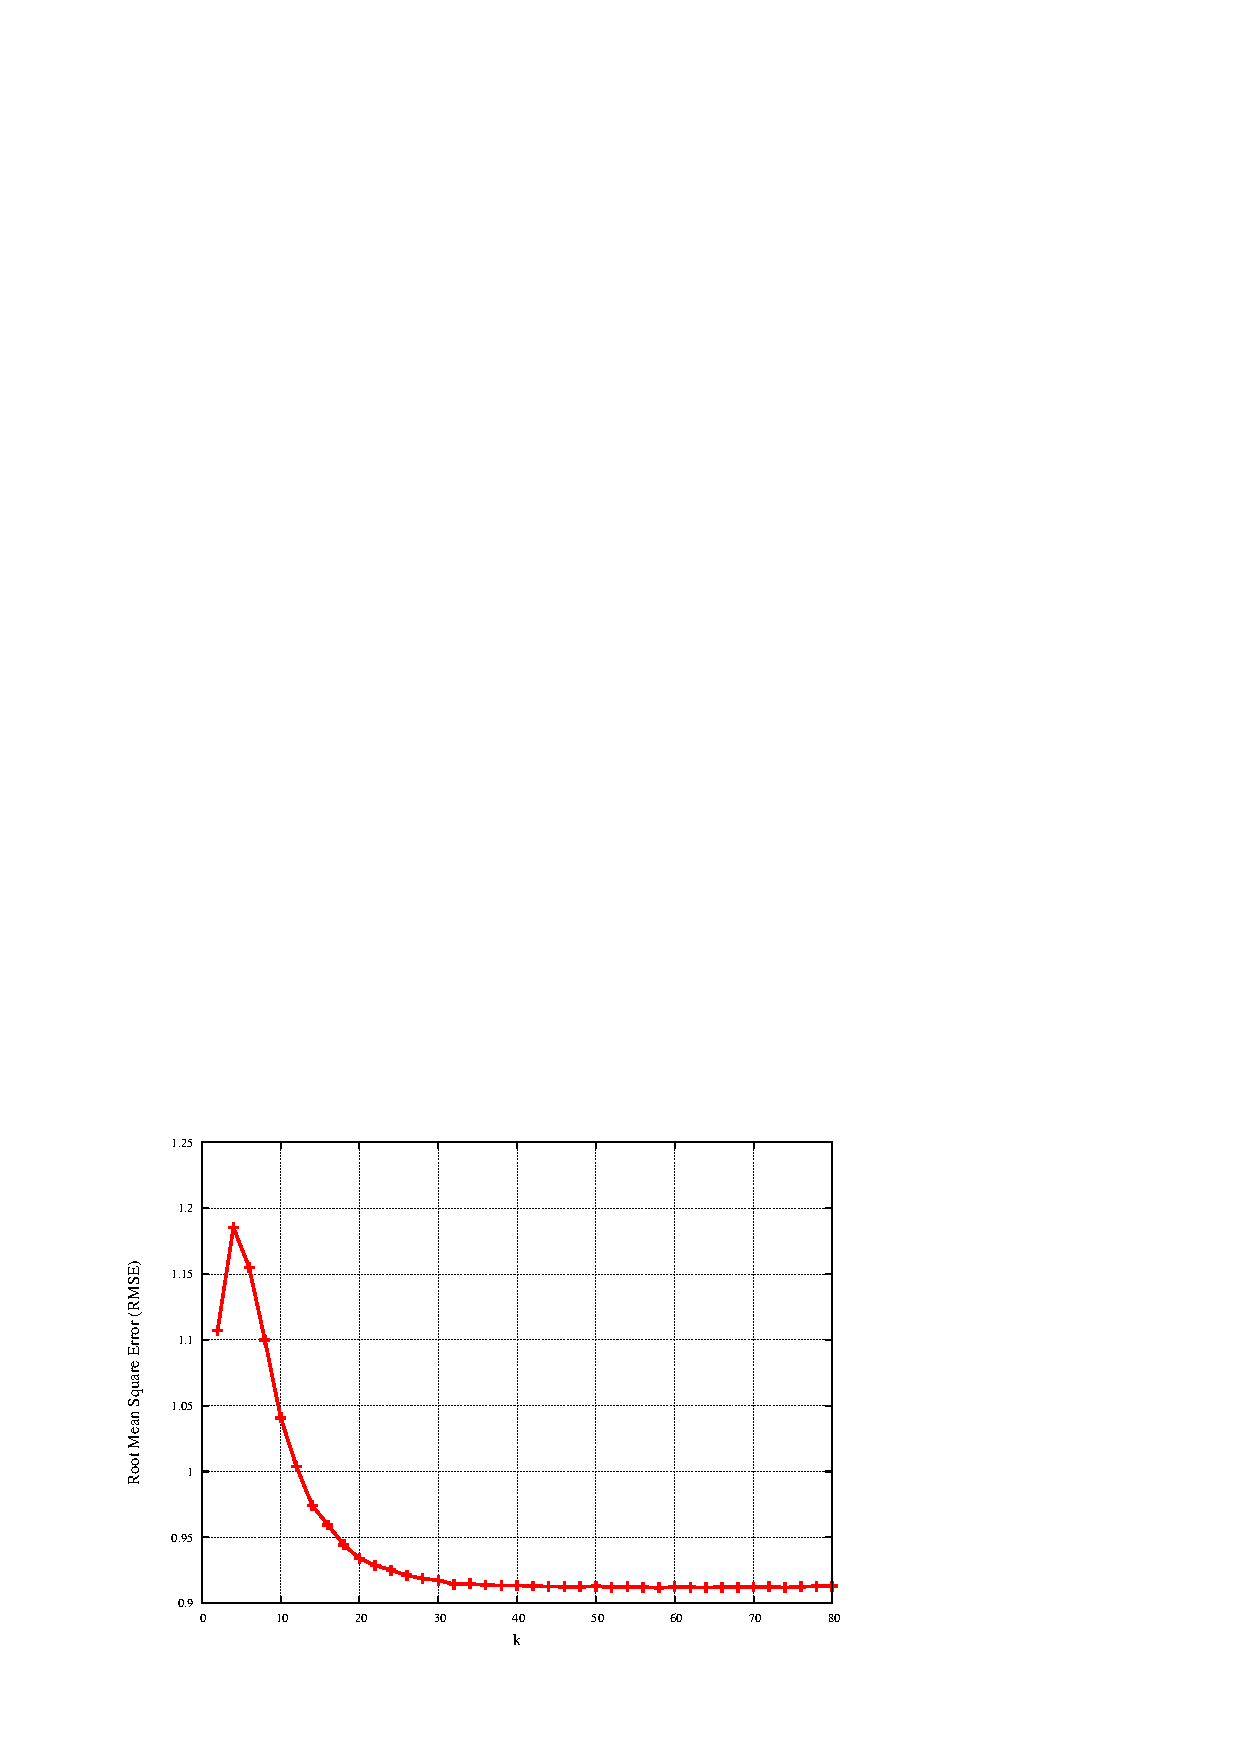
\includegraphics[scale=0.95]{figures/nocal.pdf}
	\caption[]{A plot of RMSE vs. K on our test set (all ratings excluding California businesses). Blue indicates our RMSE values when we did not use normalization; red uses normalization.}
	\label{fig:nocal}
\end{figure}


\begin{figure}[ht!]
	\centering
	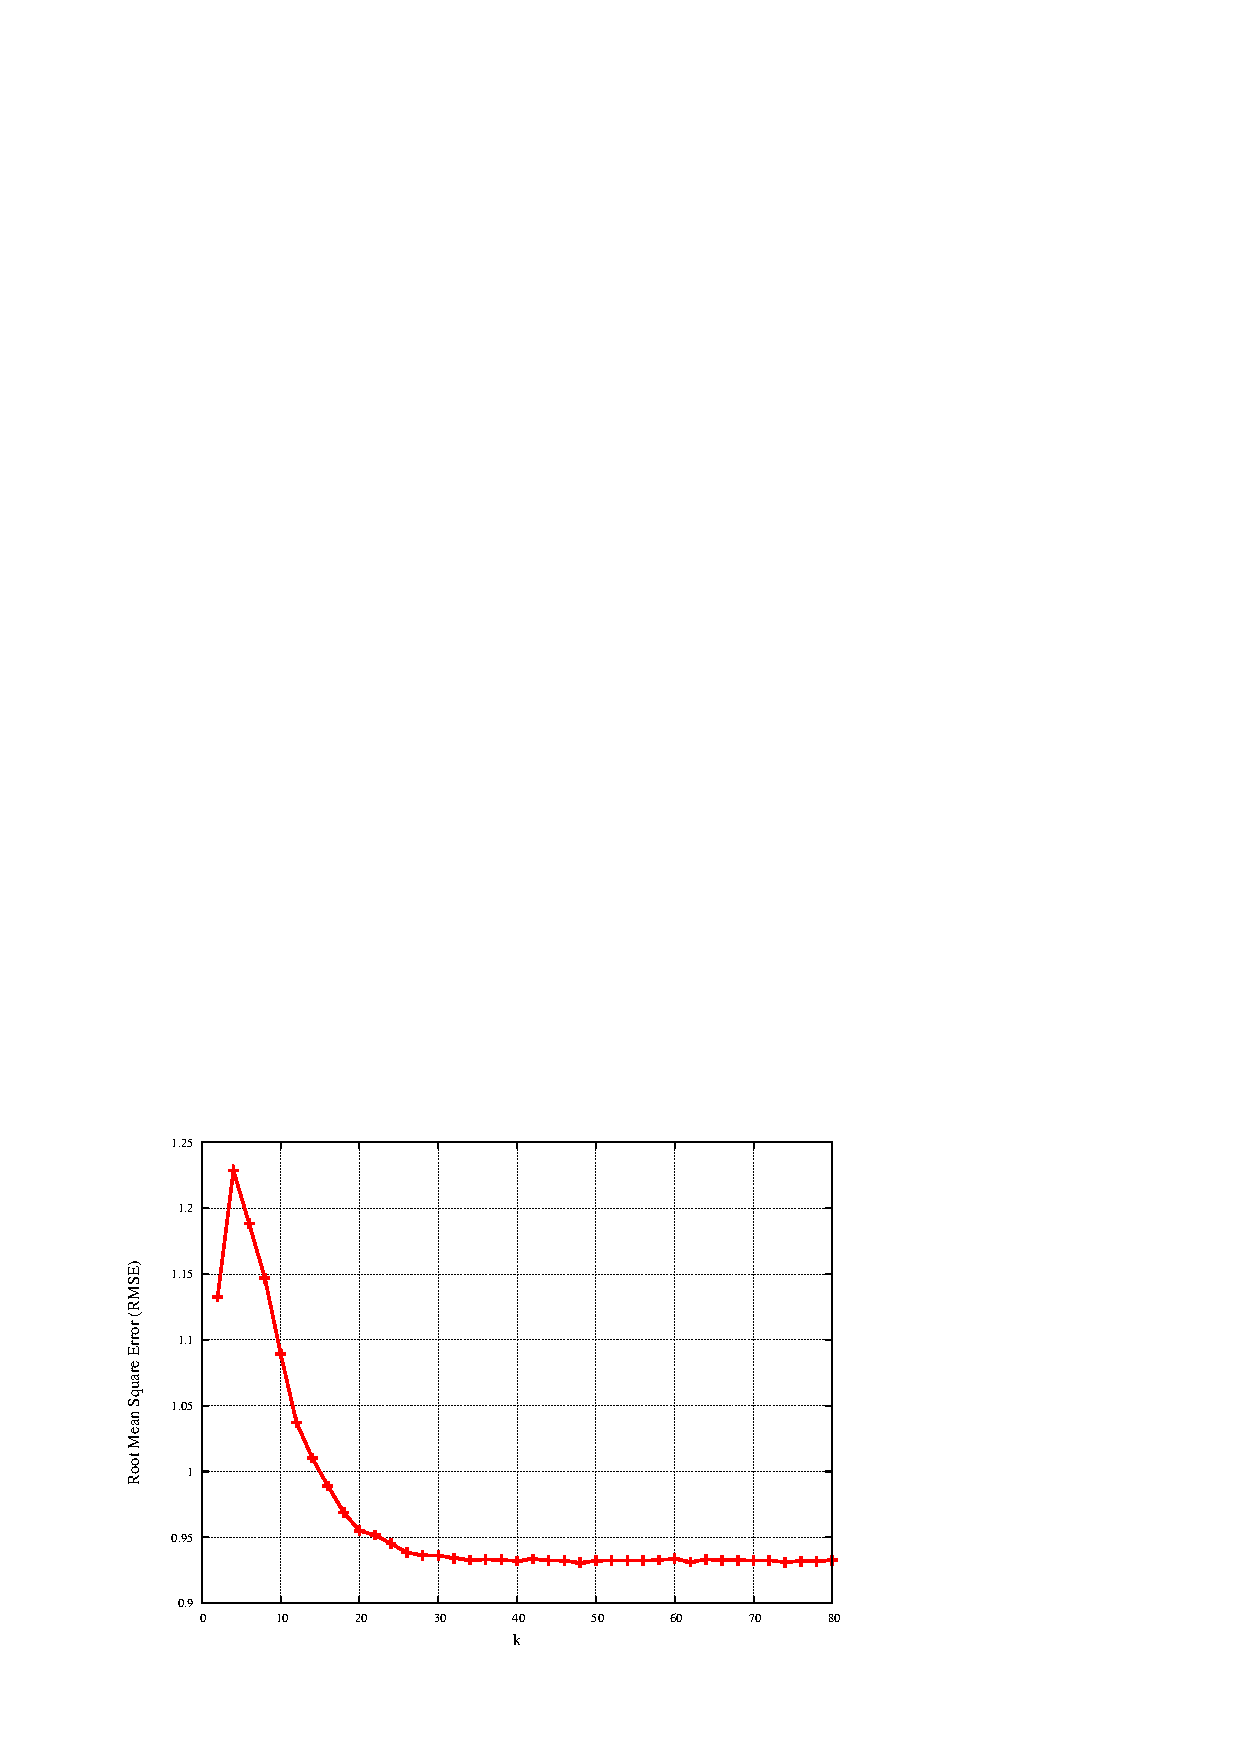
\includegraphics[scale=0.95]{figures/cal.pdf}
	\caption[]{A plot of RMSE vs. K on our evaluation set. Red indicates ratings on all California businesses and green indicates food-related business ratings in California}
	\label{fig:cal}
\end{figure}

%\begin{figure}[ht!]
%	\centering
%	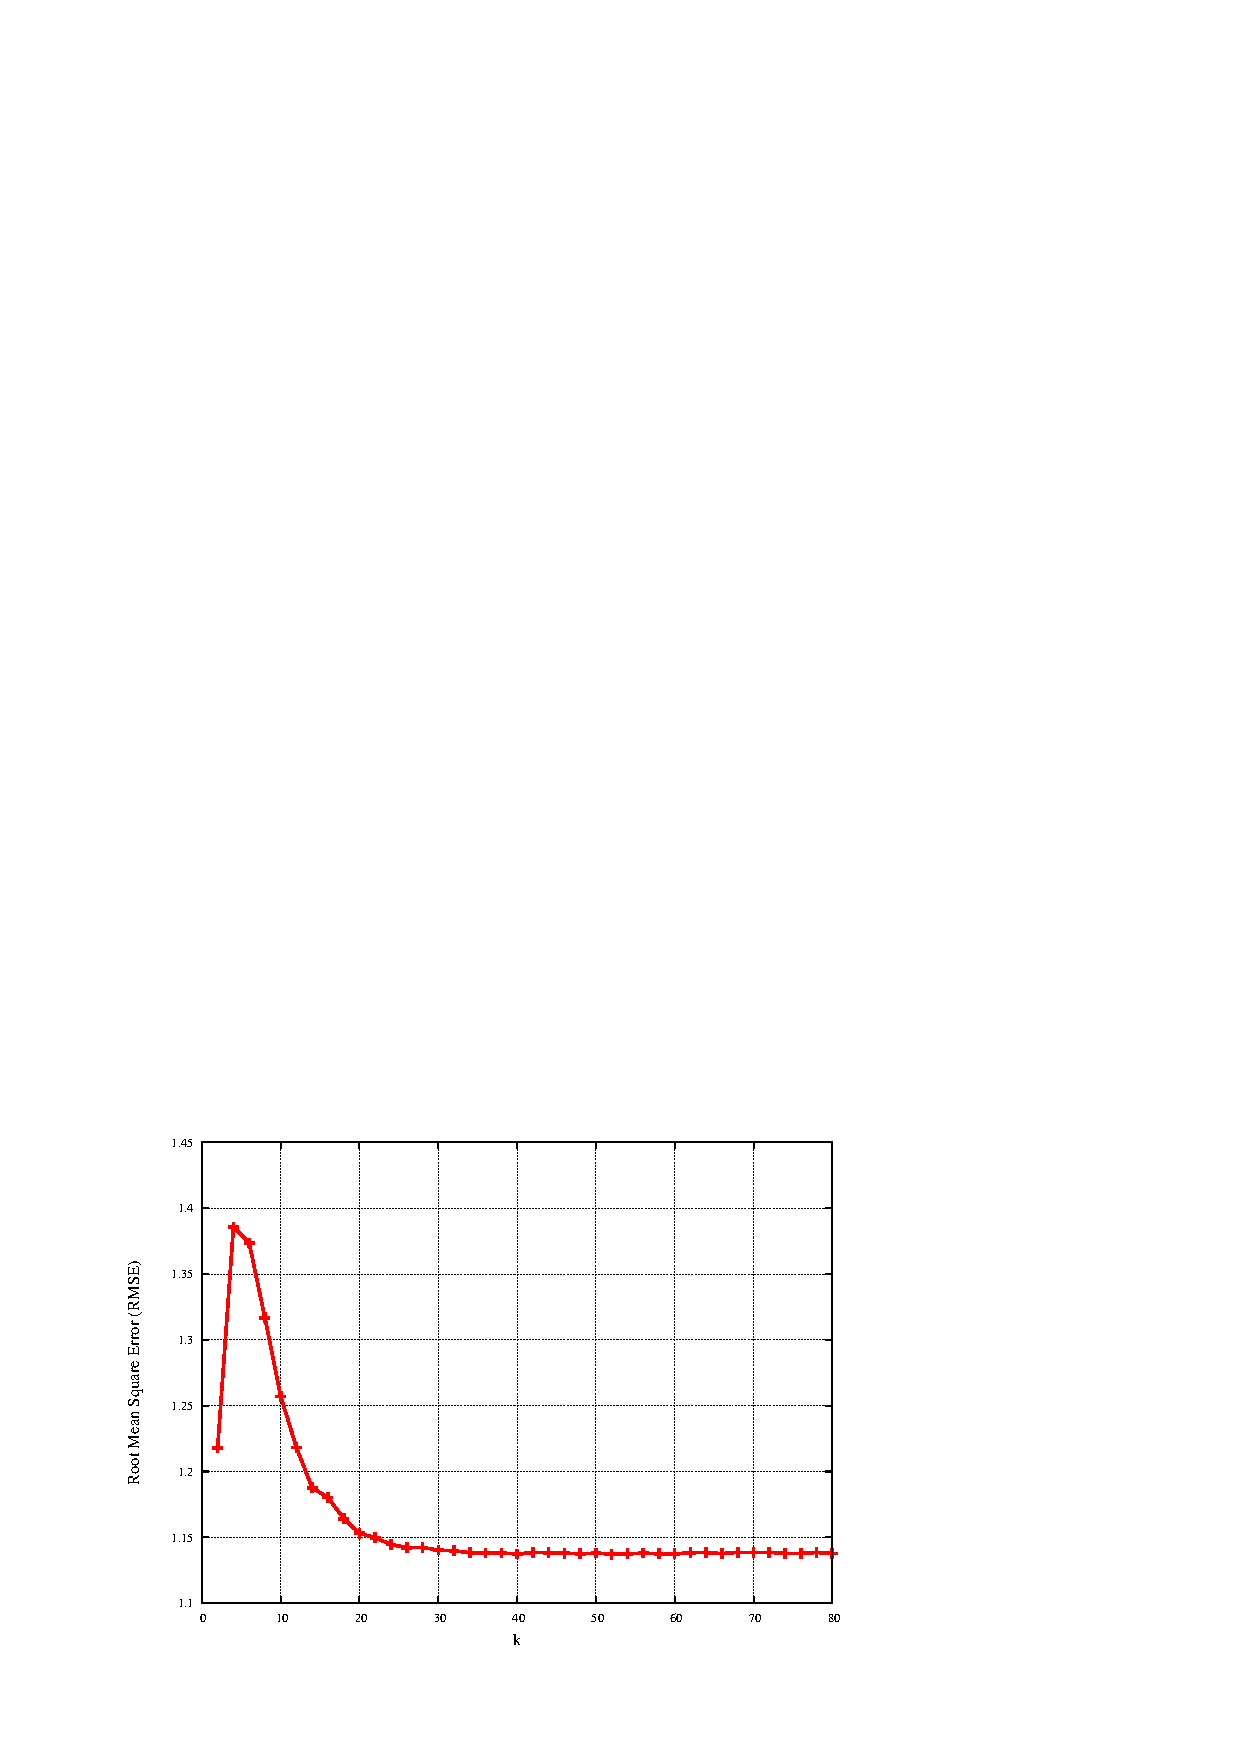
\includegraphics[scale=0.5]{figures/nocalnonorm.pdf}
%	\caption[]{A plot of RMSE vs. K for all ratings excluding 
%California businesses without normalization}
%	\label{fig:norm}
%\end{figure}

%\begin{figure}[ht!]
%	\centering
%	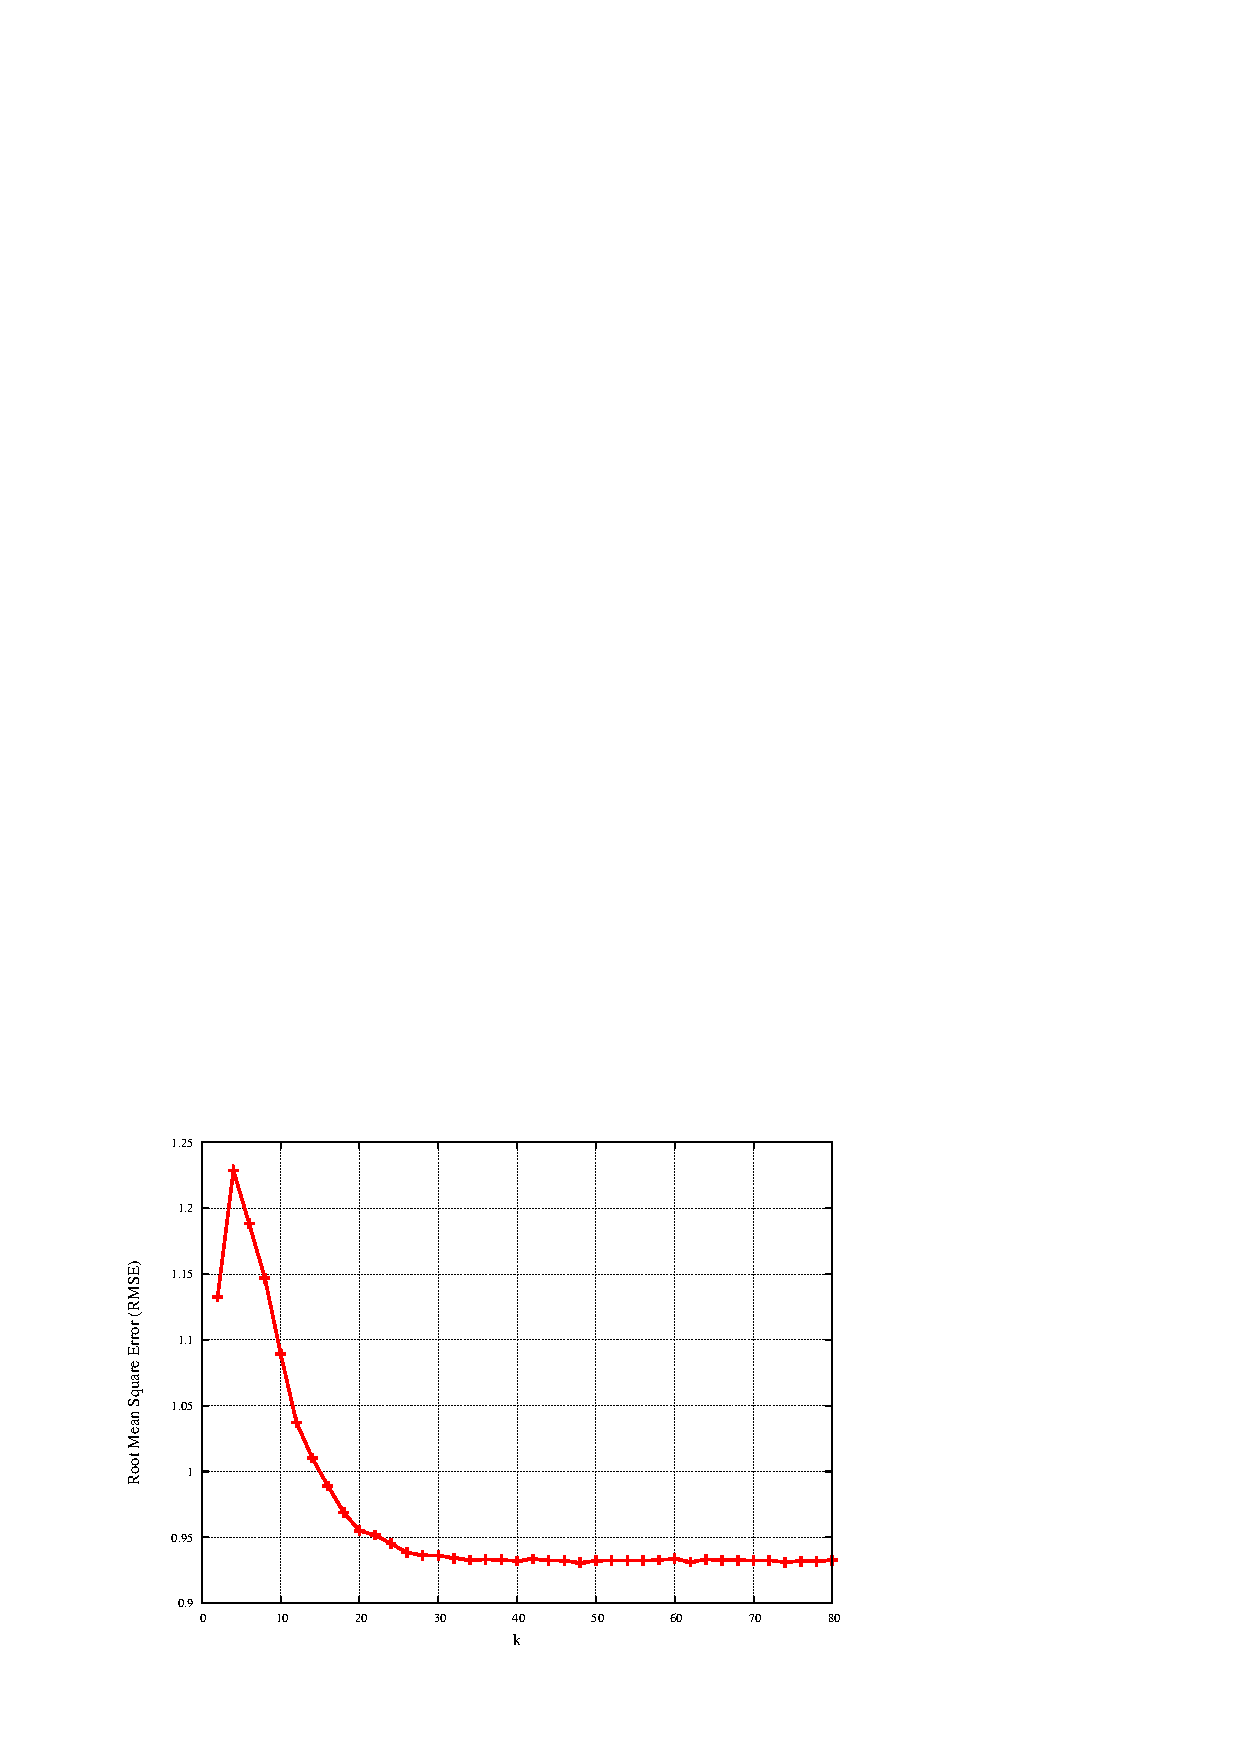
\includegraphics[scale=0.5]{figures/nocalfood.pdf}
%	\caption[]{A plot of RMSE vs. K for all food ratings excluding California businesses}
%	\label{fig:foodonly}
%\end{figure}

We also evaluated the effect of normalization by running the same tests as
above on businesses excluding California with and without a normalization
factor. Figure~\ref{fig:nocal} shows this comparison.

\subsection{Interpreting Results}
As we increase the K-values, the RMSE value approaches a minimum value which it
hovers around. For us, we were able to achieve an RMSE of \bestRMSE when
K=\bestK.
What's particularly interesting about our result is that it shows predictions
across a wide variety of businesses-genres can be useful in predicting
interests in unrelated genres. For example, predictions for clothing shops can
be used to help predict where you might like to go out to eat. We initially
thought that using unrelated businesses to predict one another would yield to
inaccurate results. However, when we excluded non-food related ratings from the
dataset, we achieved a much worse RMSE of 1.15. Figure~\ref{fig:cal} shows this comparison.

As we mentioned in Section~\ref{sec:problem}, our system is intended to be a recommendation system. 
Therefore, we care more that users are accurately informed of businesses that they will actually enjoy rather than
telling users about low rated businesses. This implies that we don't differentiate between high ratings. Our recommendation
 predictions
indicate we were successful \posAccuracy of the time. The converse of this means
that \posInaccuracy of the time we predicted a user would give at least a 3 when the actual rating was at most a 2.  For future work,
we would like to improve the accuracy of predicting positive reviews. We suspect the inaccuracy we've experienced thus far stems
from poor, abnormal, experiences at a business for  (e.g. the waiter dropped a glass of water on me).

We also compared our results to the winners of the Netflix prize,
\cite{netprize}. Unlike our technique, the winners of the Netflix prize used a
combination of different predictors working in unison to build a prediction
engine. Ideally, we would build additional prediction engines to supplement
ours. However, we were not able to do this due to time constraints. Overall,
the winners of the Netflix prize achieved an RMSE value of \bestNetflixRMSEnsp,
which is roughly \netDiff from our best RMSE of \bestRMSEnsp. When we compare against their best 
single-predictor's RMSE (0.889), the difference between our accuracy and theirs
is lowered to 0.04. However, even if we used the winning Netflix prize prediction engine,
 we feel the accuracy of 
our results would still not be as good as when it was applied to movies alone. This is likely due to
the fact that movies are much more controlled than businesses. Businesses are
affected by location, price, quality of service, and hours of operation. Movies
are always available and are displayed in a roughly uniform way. 


